\subsection{The standard BD triple}
The initial quiver is illustrated in Figure~\ref{f:h_n=3_std}. 
\begin{figure}[htb]
\begin{center}
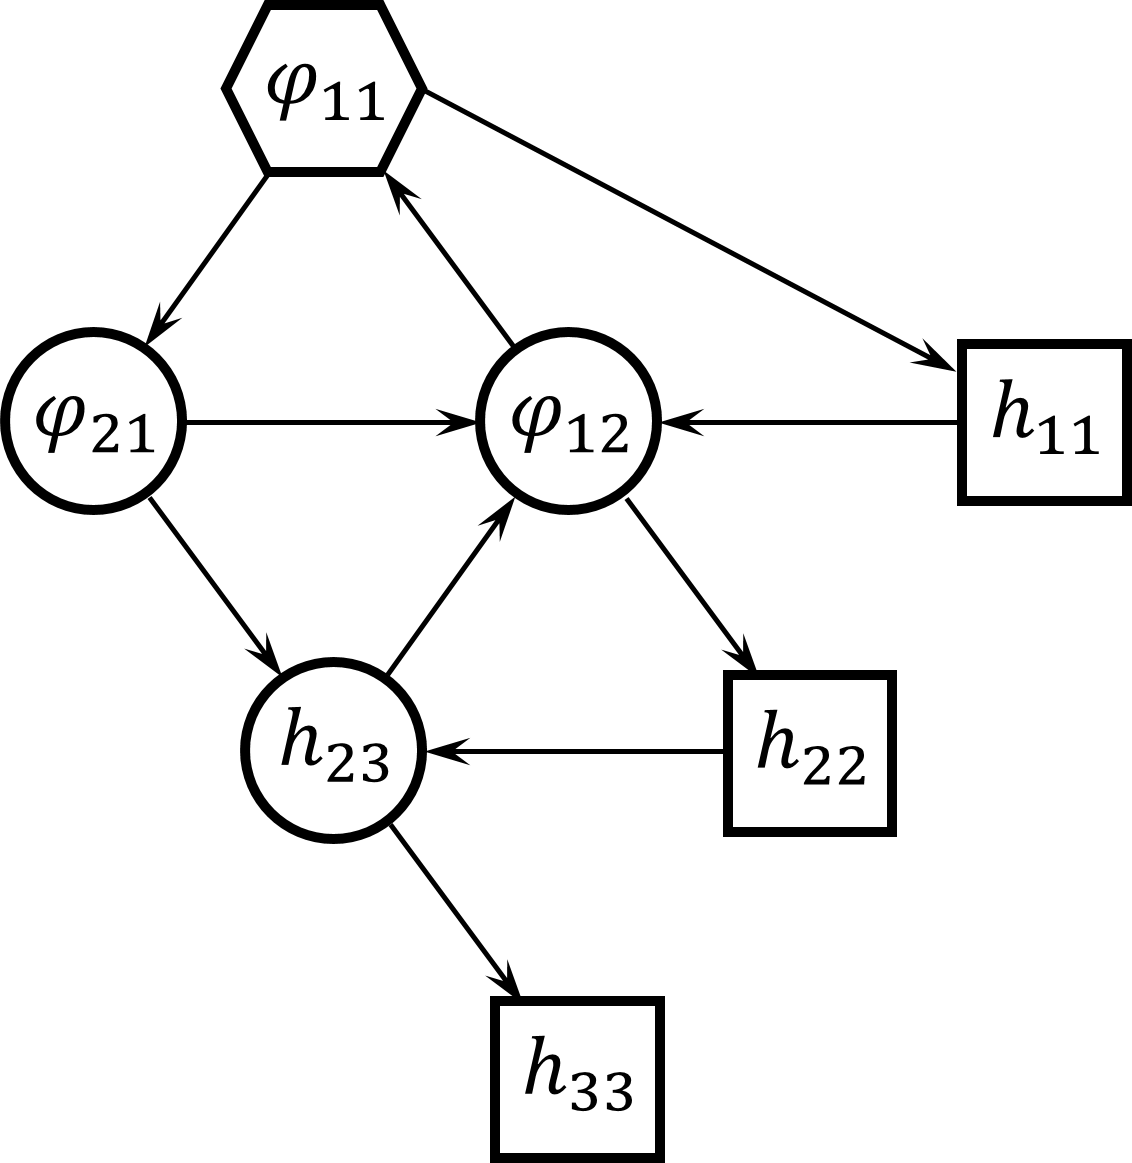
\includegraphics[scale=0.65]{h_convention/h_n=3_std.png}
\end{center}
\caption{The initial quiver for $\gc_h^{\dagger}(\bg_{\std},\GL_3)$. }
\label{f:h_n=3_std}
\end{figure}

\paragraph{The initial variables.} The variables in the initial extended cluster are given as follows:
\begin{equation}
    c_1(U) = \tr(U), \ \ c_2(U) = \frac{1}{2!} (\tr(U)^2 - \tr(U^2));
\end{equation}
\begin{equation}
    \varphi_{21}(U) = u_{13}, \ \ \varphi_{12}(U) = \det U^{[2,3]}_{[1,2]}\end{equation}\begin{equation}\varphi_{11}(U) = -\det \begin{bmatrix} u_{13} &(U^2)_{13}\\ u_{23} & (U^2)_{23}\end{bmatrix} =  u_{23}\det U^{[2,3]}_{[1,2]} + u_{13}\det U^{\{1,3\}}_{[1,2]};
\end{equation}
\begin{equation}
    h_{23}(U) = -u_{23}u_{33}-u_{13}u_{32}, \ \ h_{22}(U) = u_{33}\det U^{[2,3]}_{[2,3]} + u_{32}\det U^{[2,3]}_{\{1,3\}};
\end{equation}
\begin{equation}
    h_{11}(U) = \det U, \ \ h_{33}(U) = u_{33}.
\end{equation}

\paragraph{Some $1$-step mutations.} 
\begin{equation}
    \varphi_{11}^\prime(U) = \det \begin{bmatrix} u_{12} & u_{13}\\ (U^2)_{12} & (U^2)_{13}\end{bmatrix} = u_{12} \det U_{[1,2]}^{[2,3]} + u_{13} \det U_{\{1,3\}}^{[2,3]}.
\end{equation}